%\vspace{-4mm}

\section{Empirical Results on Pre-trained DNNs}
\label{sxn:emp}

Here, we summarize our results for the VGG and ResNet series of models.
See Appendix~\ref{sxn:appendix-addl-empirical} for additional empirical results on other models.

We only consider Linear and 2D Convolutional (Conv2D) layers because we will only examine series of commonly
available, open source, pre-trained DNNs with these kinds of layers.  All models have
been trained on ImageNet, and reported test accuracies are available.  For our analysis, we do not needs to retrain these
models--and we do not even need the test data!

\paragraph{VGG and VGG\_BN Models.}

\begin{figure*}[t] %[!htb]
   \centering
   \subfigure[log Frobenius norm $\langle\log\Vert\mathbf{W}\Vert_{F}\rangle$]{
      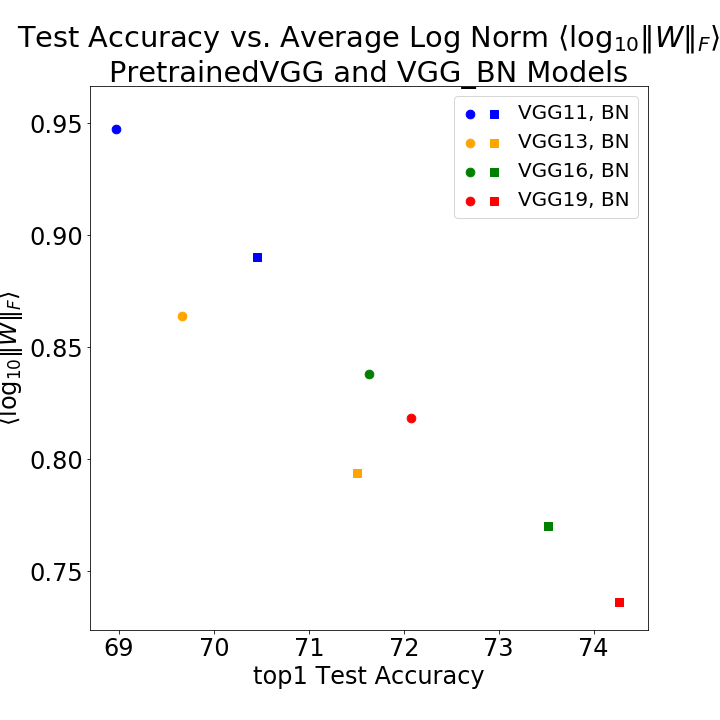
\includegraphics[scale=0.25]{img/vgg-lognorms.png}
      \label{fig:vgg_lognorms}
   }
   \subfigure[weighted average PL exponent $\hat{\alpha}$]{
      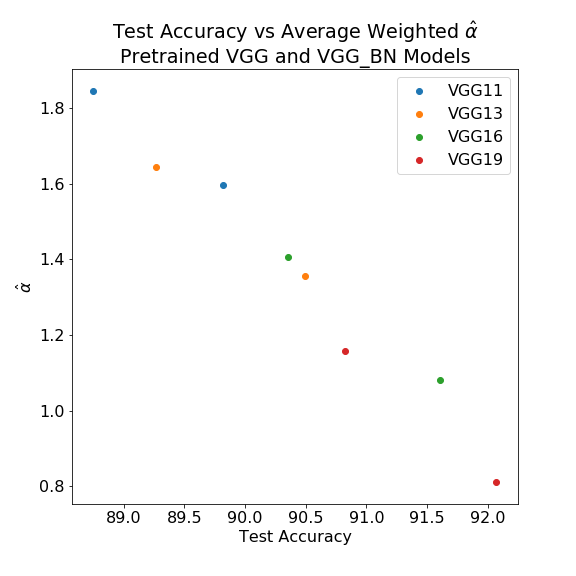
\includegraphics[scale=0.25]{img/vgg-w_alphas.png}
      \label{fig:vgg_alphahat}
   }
   \caption{%
      Pre-trained VGG and VGG\_BN Architectures and DNNs.  
      Test Accuracy versus
      average log Frobenius norm $\langle\log\Vert\mathbf{W}\Vert_{F}\rangle$ (in (\ref{fig:vgg_lognorms}))
      or
      weighted average PL exponent $\hat{\alpha}$ (in (\ref{fig:vgg_alphahat}))
      for
      VGG11 vs VGG11\_BN ({\color{blue}{blue}}),
      VGG13 vs VGG13\_BN ({\color{orange}{orange}}),
      VGG16 vs VGG16\_BN ({\color{green}{green}}),  and
      VGG19 vs VGG19\_BN ({\color{red}{red}}). 
      \michael{Charles, have circles and squares or something like that to distinguish regular and BN versions.}
   }
   \label{fig:vgg}
\end{figure*}


%% COMBINED WITH ABOVE %% \begin{figure}[!htb]
%% COMBINED WITH ABOVE %%  \centering
%% COMBINED WITH ABOVE %%    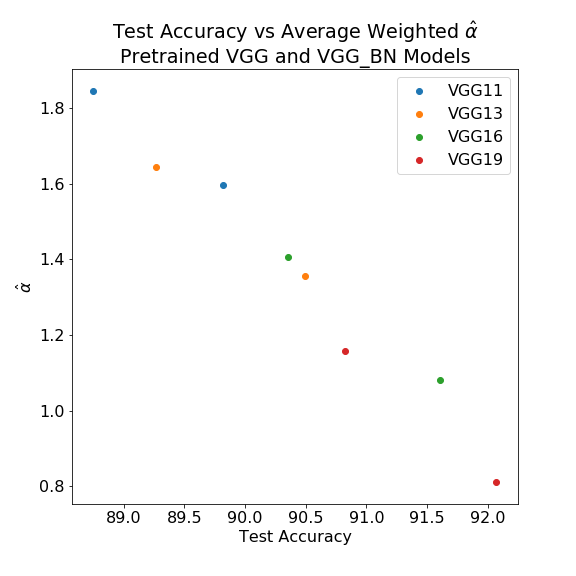
\includegraphics[scale=0.40]{img/vgg-w_alphas.png}
%% COMBINED WITH ABOVE %%    \caption{
%% COMBINED WITH ABOVE %% Pre-trained VGG and VGG BN Architectures and DNNs.  Test Accuracy and weighted average $\hat{\alpha}$ for
%% COMBINED WITH ABOVE %%  VGG11 vs VGG11\_BN ({\color{blue}{blue}}),
%% COMBINED WITH ABOVE %% VGG13 vs VGG13\_BN ({\color{orange}{orange}}),
%% COMBINED WITH ABOVE %% VGG16 vs VGG16\_BN ({\color{green}{green}}),  and
%% COMBINED WITH ABOVE %% VGG19 vs VGG19\_BN ({\color{red}{red}}). 
%% COMBINED WITH ABOVE %% }
%% COMBINED WITH ABOVE %%   \label{fig:vgg_alphahat}
%% COMBINED WITH ABOVE %% \end{figure}



\begin{table}[t]
\small
\begin{center}
\begin{tabular}{|p{0.75in}|c|c|c|c|c|c|c|}
\hline
Architecture 
 & Model &Top1 
 & Top5 & $L$ & $N_{\alpha}$ & $\hat{\alpha}$ \\
\hline
VGG11 & VGG11 & & & & & \\
  & VGG11 BN & & & & & \\
\hline
VGG13 & VGG13 & & & & & \\
  & VGG13 BN & & & & & \\
\hline
VGG16 & VGG16 & & & & & \\
  & VGG16 BN & & & & & \\
\hline
VGG19 & VGG19 & & & & & \\
  & VGG19 BN & & & & & \\
\hline
\end{tabular}
\end{center}
\caption{Results for VGG Architectures and DNN Models.}
\label{table:models_VGG}
\end{table}


We start by comparing the log Norm and Universal $\hat{\alpha}$ metrics for the  the VGG class of models.
Figure~\ref{fig:vgg} shows both the average log Frobenius norm
$\langle\log\Vert\mathbf{W}\Vert_{F}\rangle$,  Eqn.~(\ref{eqn:av_log_norm}),
and the weighted average PL exponent $\hat{\alpha}$,   Eqn.~(\ref{eqn:alpha_hat_specific}),
as a function of the reported (Top1) test accuracy for the series of pre-trained VGG models ,
as available in the pyTorch package~\cite{pyTorch}. 
These include VGG11, VGG13, VGG16, and VGG19, and
their more accurate counterparts with Batch Normalization, VGG11\_BN, VGG13\_BN, VGG16\_BN and VGG19\_BN.  
%See Figures~\ref{fig:vgg_lognorms} and~\ref{fig:vgg_alphahat} as well as Table~\ref{table:models_VGG} for details.
(See Table~\ref{table:models_VGG} for additional details.)

%Figure~\ref{fig:vgg_lognorms} shows the average log Frobenius norm results, which are quite good; and 
%Figure \ref{fig:vgg_alphahat} shows the weighted average PL exponent results, which yield slight improvements due to the method we introduce.
Across the entire series of architectures, reported test error decreases linearly with both metrics, the 
average log Frobenius norm $\langle\log_{10}\Vert\mathbf{W}\Vert_{F}\rangle$, Eqn.~(\ref{eqn:av_log_norm}), 
and the  average weighted power law exponent $\hat{\alpha}$,  Eqn.~(\ref{eqn}).
Moreover, where the log Norm relation has 2 outliers, VGG13 and VGG13\_BN, 
the Universal $\hat{\alpha}$ metric shows a near perfect linear relation across the entire VGG series.

\paragraph{ResNet Models.}

\begin{figure*}[!htb]
   \centering
   \subfigure[log Frobenius norm $\langle\log\Vert\mathbf{W}\Vert_{F}\rangle$]{
      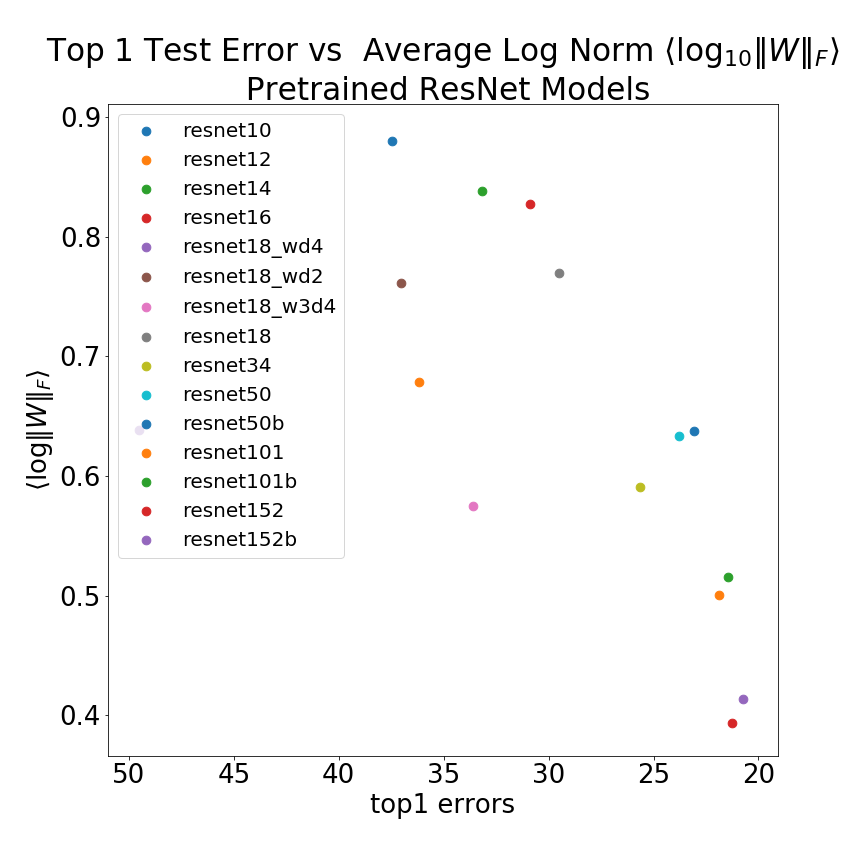
\includegraphics[scale=0.21]{img/ResNet_top1-lognorms.png}
      \label{fig:resnet_lognorms}
   }
   \subfigure[weighted average PL exponent $\hat{\alpha}$]{
      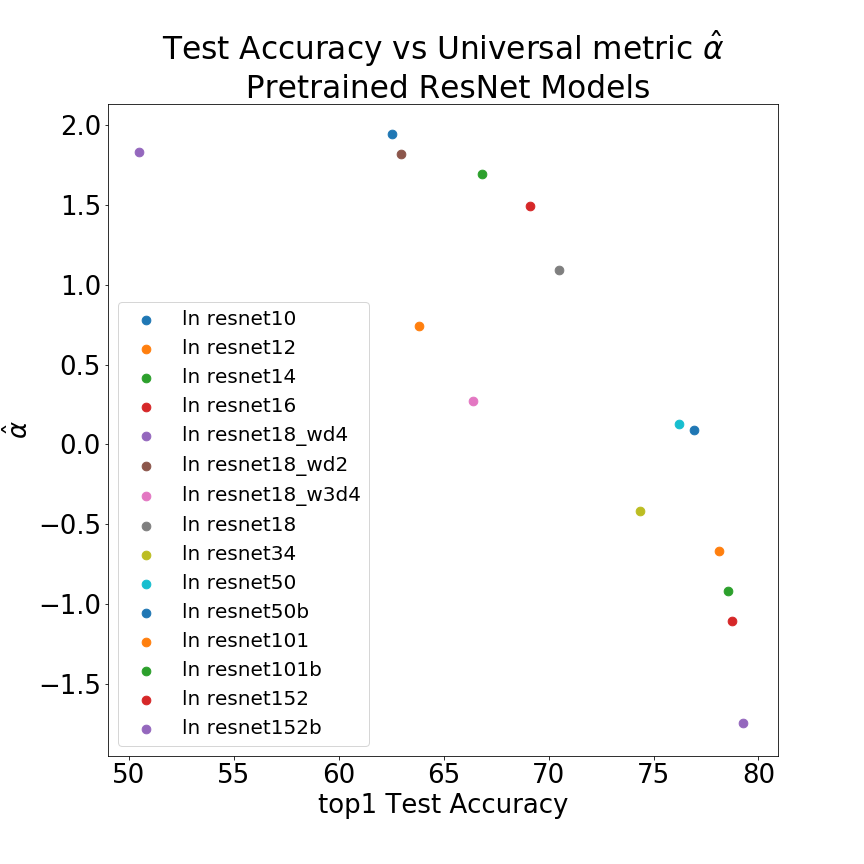
\includegraphics[scale=0.21]{img/ResNet-w_alphas.png}
      \label{fig:resnet_alphahat}
   }
   \caption{
      Pre-trained
      ResNet Architectures and DNNs.  
      Top 1 Test error versus
      average log Frobenius norm $\langle\log\Vert\mathbf{W}\Vert_{F}\rangle$ (in (\ref{fig:resnet_lognorms}))
      or
      weighted average PL exponent $\hat{\alpha}$ (in (\ref{fig:resnet_alphahat})).
           }
   \label{fig:resnet}
\end{figure*}

\begin{table}[!htb]
\small
\begin{center}
\begin{tabular}{|p{0.75in}|c|c|c|c|c|c|c|}
\hline
Architecture 
 & Model
 & Top 1 Error & $\hat{\alpha}$ \\
\hline
ResNet (small)  & resnet10 & 37.46 & \\
& resnet12 & 36.18 & \\
& resnet14 & 33.17 & \\
& resnet16 & 30.9 & \\
\hline
ResNet18 & resnet18\_wd4 & XX & \\
& resnet18\_wd2 & XX & \\
& resnet18\_wd3d4& XX & \\
& resnet18 & XX & \\

\hline
ResNet34 & resnet34 & 25.66 & \\
\hline
ResNet50 & resnet50 & 23.79 & \\
& resnet50b &  & \\

\hline
ResNet101 & resnet101 & XX.XX & \\
& resnet101b & XX.XX & \\
\hline
ResNet152 & resnet152 & XX,XX & \\
& resnet152b & XX,XX & \\
\hline
\end{tabular}
\end{center}
\caption{Results for ResNet Architectures and DNN Models.
         \michael{Charles, are we going to have the same set of columns for ResNet at least that we had for VGG in the VGG table.}
        }
\label{table:models_resnet}
\end{table}

Next we look at the ResNet class of models. 
See
Figures~\ref{fig:resnet_lognorms}
and~\ref{fig:resnet_alphahat}
as well as
Table~\ref{table:models_resnet}
for details.
Here, we consider a 15 different pretrained ResNet models, of varying sizes
and accuracies, ranging from the small ResNe10 upto the largest ResNet152 models,
as provided by the OSMR sandbox
\footnote{https://github.com/osmr/imgclsmob},
developed for  training large-scale image classification networks for embedded systems.
Again, we compare the reported (Top1) test accuracy versus the average log Norm 
$\langle\log_{10}\Vert\mathbf{W}\Vert_{F}\rangle$
and Universal $\hat{\alpha}$ metrics.

As with the VGG series, both metrics monotonically decrease as the test accuracies decreases,
both have a few large outliers off the mainline relation .  The log Norm metric has several notable outliers, 
including resnet18\_wd2, resnet18\_wd3\_d4, resnet34, and resnet10.
The $\hat{\alpha}$ relation shows a slightly better relation, with resnet18\_wd2 more in line, and
the other 3 outliers a little less off the mainline correlation.
The Universal $\hat{\alpha}$ metric is as good or slightly better than the average log Norm metric
for the Resnet series of models.  

We see similar results for our Universal PL capacity control metric $\hat{\alpha}$ across a wide ranger of  other pre-trained DNN models, 
described in the Appendix and in Table XXX.  In nearly all cases, the metric  $\hat{\alpha}$  correlates well with the reported test accuracies,
with only a three DNN architectures as exceptions.  Overall the $\hat{\alpha}$ metric systematically correlates well with the
generalization accuracy of a wide class of pre-trained DNN architectures--which is remarkable!